\documentclass{article}
\usepackage{xcolor}
\usepackage{graphicx}
\usepackage{float}
\usepackage{tikz}
\usepackage{parskip}
\usepackage{amsmath}
\usepackage{amsthm}
\usepackage{amssymb}
\usepackage{mathtools}
\usepackage{fancyhdr}
\usepackage[%paperheight = 59.4cm,
            %paperwidth = 42cm,
            %includehead,
            nomarginpar,
            textwidth=15cm,
            headheight=10mm]{geometry}


\begin{document}
 
\pagestyle{fancy}
%\fancyhead{}\fancyfoot{}

\fancyhf[OHC]{Christopher Munoz WRH3 Optimization}
\textbf{Problem 4.2:} \\
In this problem we explore descent directions for the linear function $f(x) = x_1 - 2x_2 + 3x_3$ and determine whether our solutions depend on the value of x. Let us consider the gradient of our linear function:
\begin{align*}
    \nabla f(x) = \begin{bmatrix} 1 \\ -2 \\ 3 \end{bmatrix}
\end{align*}
The descent direction is any direction that satisfies $\nabla f(x) * d < 0$ where d is a direction. Plugging in our values for our gradient we get $1d_1 - 2d_2 + 3d_3 < 0$. Note the absence of any $x$ variables, meaning our answer does not depend on our value of $x$, it must only satisfy the inequality, in our case: $1d_1 - 2d_2 + 3d_3 < 0$. This should be true for all linear functions or constant gradient.

\textbf{Problem 4.3:} Consider the following problem: 
\begin{align*}
    \text{minimize} &\null \quad f(x) = -x_1 - x_2 \\ 
    \text{subject to} &\null \quad x_1 + x_2 \leq 2 \\
     &\null \quad x_1, x_2 \geq 0
\end{align*}
We will do the following: \newline \setlength\parindent{24pt}  
\indent \{i\} Determine the feasible directions at  $x = (0,0)^T, (0,1)^T, (1,1)^T$ and $(0,2)^T$ \newline 
\indent \{ii\} Determine whether there exist feasible descent direction at these points, and hence determine which (if any) of the point can be local minimizers. 
\newline 
\begin{figure}[H]
    \centering
    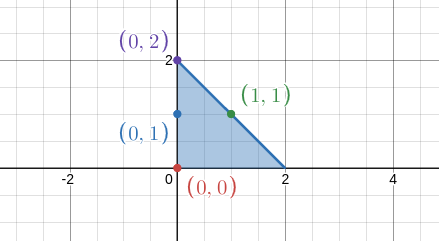
\includegraphics[scale = 0.40]{desmos2.png}
\end{figure}
\indent \textbf{\{i\}} Solution, below we let $p$ be a set of vectors.
\begin{align*}
    \bar{x} = (0,0)^T: &\null \quad \{p \in \mathbb{R}^2 | p_1 \geq 0, p_2 \geq 0 \} \\
    \bar{x} = (0,1)^T: &\null \quad \{p \in \mathbb{R}^2 | p_1 \geq 0, p_1 \leq 1 \} \\
    \bar{x} = (1,1)^T: &\null \quad \{p \in \mathbb{R}^2 | p_1 \leq 1,  p_2 \leq 1 \} \\
    \bar{x} = (0,2)^T: &\null \quad \{p \in \mathbb{R}^2 | p_1 \geq 0, p_2 \leq 2 \} \\
\end{align*}
\indent \textbf{\{ii\}} \newline For the point $(0,0)^T$, every direction $p_1 \geq 0$ and $p_2 \geq 0$ is a feasible descent direction. Its not a local minimizer. \newline
For the point $(0,1)^T$, there are feasible directions if $0 \leq p_1 $ such that $p_1 + p_2 \leq 2$, not a local minimizer. \newline
For point $(1,1)$, there are no feasible descent directions, this is local minimizer \newline
For point $(0,2)$ there are no feasible descent directions, also a local minimizer \newline

\noindent
\textbf{Problem 6.4:} We find the first three terms of the taylor series at point $x_0 = (1,-1)^T$ for:
\begin{align*}
    f(x_1, x_2) = 3x_1^4 - 2x_1^3x_2 - 4x_1^2x_2^2 + 5x_1x_2^3 + 2x_2^4
\end{align*}
We first start with finding the gradient, our partial derivatives with respect to $x_1$ then $x_2$.
\begin{align*}
    \nabla f(x) = 
    \begin{pmatrix}
        12x_1^3 - 6x_2x_1^2 - 8x_2^2x_1 + 5x_2^3 \\
        -2x_1^3 - 8x_2x_1^2 + 15x_2^2x_1 + 8x_2^3
    \end{pmatrix}
\end{align*}
Followed by our Hessian: 
\begin{align*}
    \nabla^2 f(x) = 
    \begin{pmatrix}
        36 x_1^2 - 12 x_2 x_1 - 8 x_2^2 & -6 x_1^2 - 16 x_2 x_1 + 15 x_2^2 \\
        -6 x_1^2 - 16 x_2 x_1 + 15 x_2^2 & -8 x_1^2 + 30 x_2 x_1 + 24 x_2^2
    \end{pmatrix}
\end{align*}
At the point $x_0 = (1,-1)$ our original function, gradient and Hessian have the following values:
\begin{align*}
    f(1,-1) = -2 && 
    \nabla f(1,-1) =
    \begin{pmatrix}
        5 \\ 13
    \end{pmatrix} &&
    \nabla^2 f(1,-1) = 
    \begin{pmatrix}
        40 & 25 \\
        25 & -14
    \end{pmatrix}
\end{align*}
We then plug into our general form formula for second-order Taylor expansion \newline $f(x_1, x_2) \approx f(a) + \nabla f(a)^T (x-a)+\frac{1}{2}(x-a)^T \nabla^2 (a)(x-a)$ to get our approximation:
\begin{align*}
    f(1,-1) & \approx 
    -2 + 
    \begin{pmatrix} 5 \\ 13 \end{pmatrix}
        \begin{pmatrix} x_1-1 \\ x_2 + 1 \end{pmatrix} 
            + \frac{1}{2}(x_1-1 \: x_2+1)
            \begin{pmatrix}
                40 & 25 \\
                25 & -14
            \end{pmatrix}
        \begin{pmatrix} x_1-1 \\ x_2 + 1 \end{pmatrix}
\end{align*}
Evaluating the series for $f(x_0 + p)$ gives us the value $-1.81621$. Now we compare this to our series form:
\begin{align*}
    f(1.01,-0.99) & \approx 
    -2 + 
    \begin{pmatrix} 5 \\ 13 \end{pmatrix}
        \begin{pmatrix} 0.1 \\ 0.01 \end{pmatrix} 
            + \frac{1}{2}(0.1 \: 0.01)
            \begin{pmatrix}
                40 & 25 \\
                25 & -14
            \end{pmatrix}
        \begin{pmatrix} 0.1 \\ 0.01 \end{pmatrix} \\
            & = -2 +0.63 - \frac{1}{2}0.4486 \\ 
            & = -1.1457
\end{align*}
Which is not close enough to -1.81621 for my liking so I screwed up somewhere. \newline \break
\textbf{Problem 6.5}: For the function $f(x_1, x_2) = \sqrt{x_1^2 + x_2^2}$, we find the first three terms of the Taylor series at point $x_0 = (3.4)^T$, below are our computed Gradient and Hessian:
\begin{align*}
    \nabla f(x) = 
    \begin{pmatrix}
        \frac{x_1}{\sqrt{x_1^2 + x_2^2}} \\  \frac{x_2}{\sqrt{x_1^2 + x_2^2}}
    \end{pmatrix} && 
    \nabla^2 f(x) =
    \begin{pmatrix}
        \frac{1}{\sqrt{x_1^2 + x_2^2}} - \frac{x_1^2}{(x_1^2 + x_2^2)^{3/2}} & \frac{-x_1 x_2}{(x_1^2 + x_2^2)^{3/2}} \\
        \frac{-x_1 x_2}{(x_1^2 + x_2^2)^{3/2}} & \frac{1}{\sqrt{x_1^2 + x_2^2}} - \frac{x_2^2}{(x_1^2 + x_2^2)^{3/2}}
    \end{pmatrix}
\end{align*}
Now we can compute our terms and get our taylor expansion:
\begin{align*}
    f(3, 4) = 5 && \nabla f(3,4) = (\frac{3}{5},\frac{4}{5})^T && 
    \nabla^2 f(3,4) = \begin{pmatrix} \frac{16}{125} & -\frac{12}{125} \\ -\frac{12}{125} & \frac{16}{125} \end{pmatrix}
\end{align*}
Which gets us:
\begin{align*}
    f(x_1, x_2) \approx 5 + \begin{pmatrix} \frac{3}{5} \\ \frac{4}{5} \end{pmatrix}  
            \begin{pmatrix}
                x_1 - 3 \\ x_2 - 4
            \end{pmatrix} + \frac{1}{2} 
            \begin{pmatrix}
                x_1 - 3 \\ x_2 - 4
            \end{pmatrix}
            \begin{pmatrix} \frac{16}{125} & -\frac{12}{125} \\ -\frac{12}{125} & \frac{16}{125} \end{pmatrix}
            \begin{pmatrix}
                x_1 - 3 \\ x_2 - 4
            \end{pmatrix}
\end{align*} This is our taylor expansion \newline
\textbf{Problem 6.6} Theorem: If $ p^T \nabla f(x_k) < 0$ then $f(x_k + \epsilon p) < 0$ for $\epsilon > 0$
\proof First we expand $f(x_k + \epsilon p)$ in a Taylor series about the point $x_k$
\begin{align*}
    f(x_k + \epsilon p) \approx f(x_k) + (\epsilon p)^t \nabla f(x_0) + \frac{1}{2} (\epsilon p )^T \nabla^2 f(x_k)(\epsilon p)
\end{align*}
because $\epsilon$ is super tiny, the quadratic terms becomes negligible compared to the linear terms because  $\epsilon$ is multiplyed by itself in the quadratic term, we can remove that term and do the following:
\begin{align*}
    f(x_k + \epsilon p) & \approx f(x_k) + (\epsilon p)^t \nabla f(x_0) \\
    f(x_k + \epsilon p) - f(x_k) & \approx (\epsilon p)^t \nabla f(x_0)
\end{align*}
since $ p^T \nabla f(x_k) < 0$ or negative and $\epsilon > 0$ or positive, $(\epsilon p)^t \nabla f(x_0) < 0$, Thus:
\begin{align*}
    f(x_k + \epsilon p) - f(x_k) & \approx (\epsilon p)^t \nabla f(x_0) < 0 \\
    f(x_k + \epsilon p) - f(x_k) & < 0 \\
    \null && \qedsymbol
\end{align*} \\ 
\textbf{Problem 1.2} We consider the set defined by the constraints $x_1 + x_2 = 1, x_1 \geq 0, x_2 \geq 0 $ at the points (a)$(0,1)^T$; (b)$(1,0)^T$ and (c)$(0.5)(0.5)^T$ and determine the feasible directions, let $p$ be a set of vectors in $\mathbb{R}^2$:

\noindent(a) For the point $(0,1)^T$, our only feasible direction is on the line at the end in one direction increasing our $x_1$ and decreasing our $x_2$. in order to stay within our constraints: \newline $\{p \in \mathbb{R}^2 | p_1 = -p_2, p_1 \geq 0, p_2 \leq 1\}$ 

\noindent(b) For the point $(1,0)^T$ we run into a similar case where our only feasible direction is on the line, decreasing our $x_1$ while increasing our $x_2$, in order to stay within our constraints: \newline $\{p \in \mathbb{R}^2 | -p_1 = p_2, p_1 \leq 1, p_2 \geq 0\}$

\noindent(c) For the point $(0.5,0.5)^T$ we are also bounded to the line, we're right in the middle of it. We can move in 2 directions , up and down the line where $p_1 = -p_2$. We'll be more explicit about our constraint: $\{p \in \mathbb{R}^2 | p_1 + p_2 = 0\}$
\newline
\newline
\textbf{Problem 1.3} We consider the system of inequality constraints $Ax \geq b$:
\begin{align*}
    A =
    \begin{pmatrix}
        9 & 4 & 1 & 9 & -7 \\
        6 & -7 & 8 & -4 & -6 \\ 
        1 & 6 & 3 & -7 & 6
    \end{pmatrix} && 
    \text{ and }
    b =
    \begin{pmatrix}
        -15 \\ -30 \\ -20
    \end{pmatrix}
\end{align*} We will perform a ratio test $\bar{\alpha} = \min(A^T\bar{x} - b_i) / (-\alpha_i^T p)$ to determine the max step length $\bar{\alpha}$ such that $x + \bar{\alpha} p$ remains feasible for the following values of $x$ and $p$:

\noindent(i) $x =  (8,4,-3,4,1)^T$ and $p = (1,1,1,1,1)^T$ 
\begin{align*}
    Ax = \begin{pmatrix}
        9 & 4 & 1 & 9 & -7 \\
        6 & -7 & 8 & -4 & -6 \\ 
        1 & 6 & 3 & -7 & 6
    \end{pmatrix}
    \begin{pmatrix}
        8 \\ 4 \\ -3 \\ 4 \\ 1
    \end{pmatrix} = \begin{pmatrix}
        114 \\ -26 \\ 1
    \end{pmatrix} \\
    Ap = \begin{pmatrix}
        9 & 4 & 1 & 9 & -7 \\
        6 & -7 & 8 & -4 & -6 \\ 
        1 & 6 & 3 & -7 & 6
    \end{pmatrix}
    \begin{pmatrix}
        1 \\ 1 \\ 1 \\ 1 \\ 1
    \end{pmatrix} = \begin{pmatrix}
        16 \\ -3 \\ 9
    \end{pmatrix} \\
    b - Ax = \begin{pmatrix}
        -15 \\ -30 \\ 20  
    \end{pmatrix} -
    \begin{pmatrix}
        114 \\ -26 \\ 1
    \end{pmatrix} =
    \begin{pmatrix}
        -129 \\ -4 \\ 19
    \end{pmatrix} 
\end{align*}
Now we can begin to solve the inequality for $\bar{a} \geq \frac{b - Ax}{Ap}$ note that $\bar{\alpha}$ needs to be non-negative for there to be a feasible step.
\begin{align}
    \bar{a} &\geq \frac{-129}{16} \approx -8.0625 \\
    \bar{a} & \geq \frac{-4}{-3} \approx 1.333\bar{3} \\
    \bar{a} & \geq \frac{19}{9} \approx 2.111\bar{1}
\end{align}

Thus we find the maximum step length to be $\bar{a} \approx 2.111\bar{1}$

\setcounter{equation}{0}

\noindent(ii) $x = (7,-4,-3,-3,3)^T$ and $p = (3,2,0,1,-2)^T$
\begin{align*}
    Ax = \begin{pmatrix}
        9 & 4 & 1 & 9 & -7 \\
        6 & -7 & 8 & -4 & -6 \\ 
        1 & 6 & 3 & -7 & 6
    \end{pmatrix}
    \begin{pmatrix}
        7 \\ -4 \\ -3 \\ -3 \\ 3
    \end{pmatrix} = \begin{pmatrix}
        -4 \\ 40 \\ 13
    \end{pmatrix} \\
    Ap = \begin{pmatrix}
        9 & 4 & 1 & 9 & -7 \\
        6 & -7 & 8 & -4 & -6 \\ 
        1 & 6 & 3 & -7 & 6
    \end{pmatrix}
    \begin{pmatrix}
        3 \\ 2 \\ 0 \\ 1 \\ -2
    \end{pmatrix} = \begin{pmatrix}
        58 \\ 12 \\ -4
    \end{pmatrix} \\
    b - Ax = \begin{pmatrix}
        -15 \\ -30 \\ 20  
    \end{pmatrix} -
    \begin{pmatrix}
        -4 \\ -40 \\ 13
    \end{pmatrix} =
    \begin{pmatrix}
        -11 \\ -10 \\ 7
    \end{pmatrix} 
\end{align*}
\begin{align}
    \bar{a} &\geq \frac{-11}{58} \approx -0.1896 \\
    \bar{a} & \geq \frac{-10}{12} \approx -0.833\bar{3} \\
    \bar{a} & \geq \frac{7}{-4} \approx -1.7500
\end{align}
There are no feasible step, all these values are negative.

\setcounter{equation}{0}
\noindent(iii) $x = (5, 0,-6,-8,3)^T$ and $p = (5,0,5,1,3)^T$
\begin{align*}
    Ax = \begin{pmatrix}
        9 & 4 & 1 & 9 & -7 \\
        6 & -7 & 8 & -4 & -6 \\ 
        1 & 6 & 3 & -7 & 6
    \end{pmatrix}
    \begin{pmatrix}
        5 \\ 0 \\ -6 \\ -8 \\ -3
    \end{pmatrix} = \begin{pmatrix}
        -12 \\ 32 \\ 25
    \end{pmatrix} \\
    Ap = \begin{pmatrix}
        9 & 4 & 1 & 9 & -7 \\
        6 & -7 & 8 & -4 & -6 \\ 
        1 & 6 & 3 & -7 & 6
    \end{pmatrix}
    \begin{pmatrix}
        5 \\ 0 \\ 5 \\ 1 \\ 3
    \end{pmatrix} = \begin{pmatrix}
        38 \\ 48 \\ 31
    \end{pmatrix} \\
    b - Ax = \begin{pmatrix}
        -15 \\ -30 \\ 20  
    \end{pmatrix} -
    \begin{pmatrix}
        -12 \\ -32 \\ 25
    \end{pmatrix} =
    \begin{pmatrix}
        -3 \\ 2 \\ -5
    \end{pmatrix} 
\end{align*}
\begin{align}
    \bar{a} &\geq \frac{-3}{38} \approx -0.0790 \\
    \bar{a} & \geq \frac{2}{48} \approx 0.041\bar{6} \\
    \bar{a} & \geq \frac{-5}{31} \approx -0.1613
\end{align}
We find our maximum step length to be $\bar{a} \approx 0.041\bar{6}$

\setcounter{equation}{0}
\noindent(iv) $x = (9,1,-1,6,3)^T$ and $p = (-4,-2,4,-2,2)^T$
\begin{align*}
    Ax = \begin{pmatrix}
        9 & 4 & 1 & 9 & -7 \\
        6 & -7 & 8 & -4 & -6 \\ 
        1 & 6 & 3 & -7 & 6
    \end{pmatrix}
    \begin{pmatrix}
        9 \\ 1 \\ -1 \\ 6 \\ 3
    \end{pmatrix} = \begin{pmatrix}
        117 \\ -3 \\ -12
    \end{pmatrix} \\
    Ap = \begin{pmatrix}
        9 & 4 & 1 & 9 & -7 \\
        6 & -7 & 8 & -4 & -6 \\ 
        1 & 6 & 3 & -7 & 6
    \end{pmatrix}
    \begin{pmatrix}
        -4 \\ -2 \\ 4 \\ -2 \\ 2
    \end{pmatrix} = \begin{pmatrix}
        -72 \\ 18 \\ 22
    \end{pmatrix} \\
    b - Ax = \begin{pmatrix}
        -15 \\ -30 \\ 20  
    \end{pmatrix} -
    \begin{pmatrix}
        117 \\ -3 \\ -12
    \end{pmatrix} =
    \begin{pmatrix}
        -132 \\ -27 \\ 32
    \end{pmatrix} 
\end{align*}
\begin{align}
    \bar{a} &\geq \frac{-132}{-72} \approx 1.833\bar{3} \\
    \bar{a} & \geq \frac{-26}{18} \approx -1.444\bar{4} \\
    \bar{a} & \geq \frac{32}{-12} \approx -2.6666
\end{align}
We find our maximum step length to be $\bar{a} \approx 1.833\bar{3}$
\end{document}
\end{document}
